% !TeX root =../main.tex

\chapter{Fundamentals} \label{sec:fundamentals}
In this chapter, first the workings of a buck converter are discussed in section \ref{sec:the_buck_converter}. After that, the different types of losses occurring in a buck converter are explained in sections \ref{sec:losses_in_switching_elements} and \ref{sec:losses_in_the_inductor}, first focusing on the losses occurring in the switching elements and then explaining the losses occurring in the inductor. 
\section{The buck converter}
\label{sec:the_buck_converter}
DC to DC converters come in many different topologies, one of which is the synchronous buck converter seen in figure \ref{fig:synch_buck_converter_2}. Buck converters are step down converters, taking in a high voltage and outputting a low voltage. In contrast to other methods of voltage reduction, converters aim to have close to zero power loss across them. This results in the current at the output being greater than the current at the input. \\
\begin{figure}[H]
    \centering
    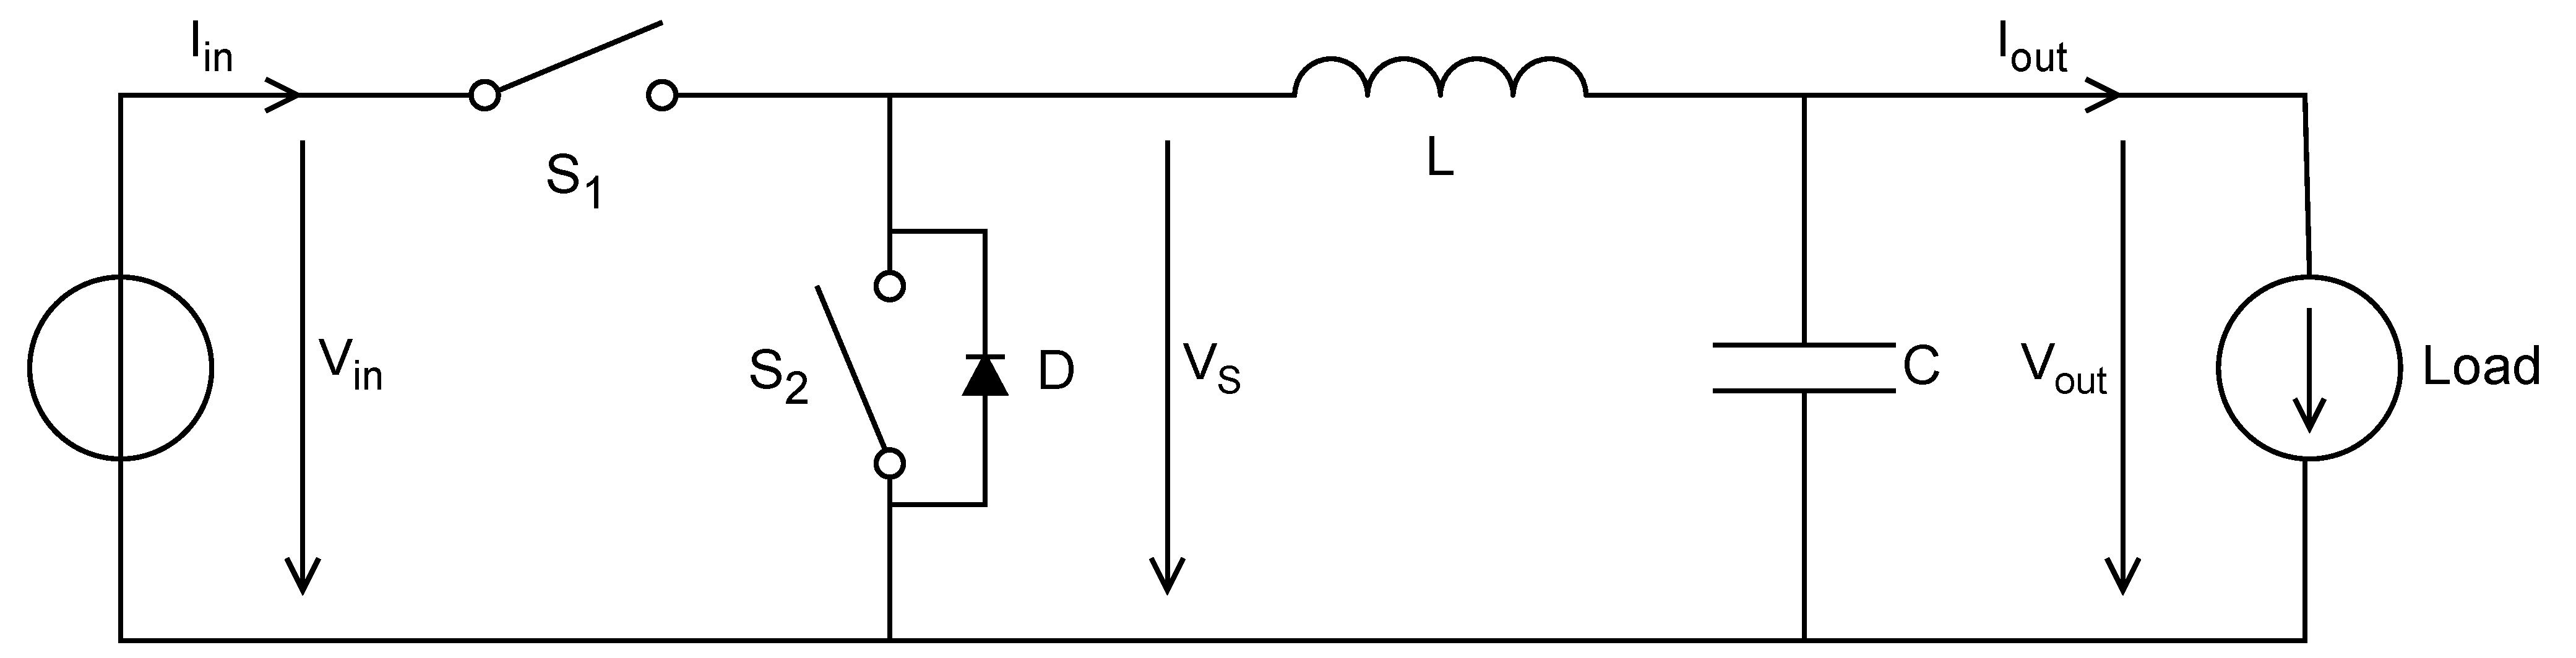
\includegraphics[width=1\linewidth]{Bilder//Kapitel2/SBC_2_D.pdf}
    \caption{Synchronous Buck Converter}
    \label{fig:synch_buck_converter_2}
\end{figure}
As shown in figure \ref{fig:stages_of_a_buck_converter.}, to function buck converters repeatedly charge and discharge the inductor $L$ by switching the two switches with a given frequency and duty cycle. Closing switch $S_1$, also refereed to the \ac{HS} switch, allows current to flow from the source to the load through the inductor. The inductor resists the change in current, charging its magnetic field while increasing the current linearly. After a certain time $t_1$, switch $S_1$ is opened, stopping the current flowing in from the source. The current through the inductor however is forced to continue flowing, now discharging the inductor through the diode D connected to the switch $S_2$, the \ac{LS} switch. To avoid short circuits, $S_2$ is not closed simultaneously with the opening of $S_1$ but is instead delayed by a dead time $t_{d}$. During dead time the negative voltage drop $V_d$ across the diode can be observed, After this dead time, switch $S_2$ is closed, and the inductor discharges for the rest of the period $T_1$. Switch $S_2$ opens again and after a second short dead time, $S_1$ connects the circuit back to the power source. The naming-convention of the dead times follows the signal supplied to the \ac{HS} switch. Opening the switch is done by the falling edge of the signal, resulting in the dead time to be named the falling edge dead time $t_{df}$. Similarly, on the rising edge of the signal to $S_1$ the dead time is called the rising edge dead time $t_{dr}$.

\begin{figure}[H]
    \centering
    \includegraphics[width=1\linewidth]{Bilder//Kapitel2/BuckConverter_Stages_1_1.pdf}
    \caption{Internal operation of a buck converter}
    \label{fig:stages_of_a_buck_converter}
\end{figure}

As long as the magnetic field of the inductor is not fully discharged by the time the \ac{HS} is closed again, the buck converter operates in \ac{CCM}. In \ac{CCM} the current through the inductor can be viewed as the superposition of two functions. First, a \ac{DC} that flows through the load labelled $I_{out}$ and secondly a triangle shaped \ac{AC}, called the ripple current $I_{L_r}$. Depending on the switching frequency, duty cycle and inductance, this ripple current can be more or less pronounced. The output capacitor is used to stabilise the current at the output gate, stopping the ripple current from reaching the load. It therefore acts as an ideal low pass filter, keeping both output current and voltage constant.\\
In real synchronous buck converters, there is no separate diode connected across the \ac{LS} switching element. Instead, both commonly used \acp{MOSFET} and \acp{GaNFET} are able to conduct reverse current, acting similarly to a diode. \\

To calculate the dependency between the output and input voltages, the current across the inductor is analysed. For any type of inductor, the relationship between inductor current and inductor voltage is given by \ref{eq:inductor_current}.
\begin{equation}\label{eq:inductor_current}
    i_L(t) = \frac{1}{L} \cdot \int_{0}^{t} v_L(\tau) \,d\tau
\end{equation}
As for constant currents, the voltage experienced by an inductor is zero, only the change in current affects the inductor voltage and therefore in turn the output voltage. The time for which a specific voltage is applied to the inductor is given by the on-time and off-time of the switch. These are characterised by the time it takes to complete an entire switching cycle $T_s$ and the fraction of that time they each take up, denoted by the duty cycle $D$.\\
For the on-time of the switch, the change in current $\Delta i_{L_{on}}$ is given by equation \ref{eq:inductor_current_on}, as the inductor's voltage is equal to the difference in voltage between the input and output gate. During the off-time, the inductors current falls as the input is no longer connected. Excluding dead time, as $T_s >> (t_{df} + t_{dr})$ the voltage across the inductor is equal to the output voltage $V_{out}$. This results in equation \ref{eq:inductor_current_off} describing the off-time current change. 
\begin{align}
    \Delta i_{L_{on}} &= \frac{1}{L} \cdot (V_{in} - V_{out}) \cdot D \cdot T_{s}       \label{eq:inductor_current_on}\\
    \Delta i_{L_{off}} &\approx \frac{1}{L} \cdot V_{out} \cdot (1-D) \cdot T_{s}     \label{eq:inductor_current_off}\\
\end{align}
For steady-state operation, the changes in the inductor current have to cancel each other out, as the current at the beginning of the cycle has to match the current at the end of it. Using this relation, given in equation \ref{eq:inductor_current_cancel}, results in equation \ref{eq:duty_cycle}. Neglecting the dead time causes the output voltage only to depend on the input voltage and the duty cycle. 
\begin{align}
    \Delta I_{L_{on}} &+ \Delta I_{L_{off}} = 0                                         \label{eq:inductor_current_cancel}\\
    D &\approx \frac{V_{out}}{V_{in}} 
        \label{eq:duty_cycle}
\end{align}


\section{Buck converter losses}\label{sec:losses_in_bc}
The synchronous buck converter's three main components, the capacitor, switching elements and inductor all contribute to power loss and are to a certain degree frequency-dependent. The capacitive losses are not discussed in great detail in this thesis, as they are usually responsible for less than 1\% of the total losses \cite{An_Accurate_Approach_for_Calculating_the_Efficiency_of_a_SBC}.
\subsection{Losses in the switching elements}\label{sec:losses_in_switching_elements}
The main causes of losses in switching elements are conductive losses, dead time losses and switching losses. Gate drive losses and capacitive losses are not explored in this thesis, as they are minimal compared with the before-mentioned causes. \\
A sixth type of loss, the reverse recovery loss resulting from the body diode of \acp{MOSFET}, does not play a role in this thesis, as it focuses exclusively on \acp{GaNFET}, which lack a body diode. This, however, does not exempt \acp{GaNFET} from conducting a current in reverse. Applying a negative drain-source voltage $V_{DS}$ results in diode-like behaviour, inducing a negative drain-source current $I_{DS}$. To model this, a diode is incorporated into the \ac{ECM} as shown in figure \ref{fig:GaNFET_ECM} \cite{Does_GaN_Have_a_Body_Diode}.
\begin{figure}[H]
    \centering
    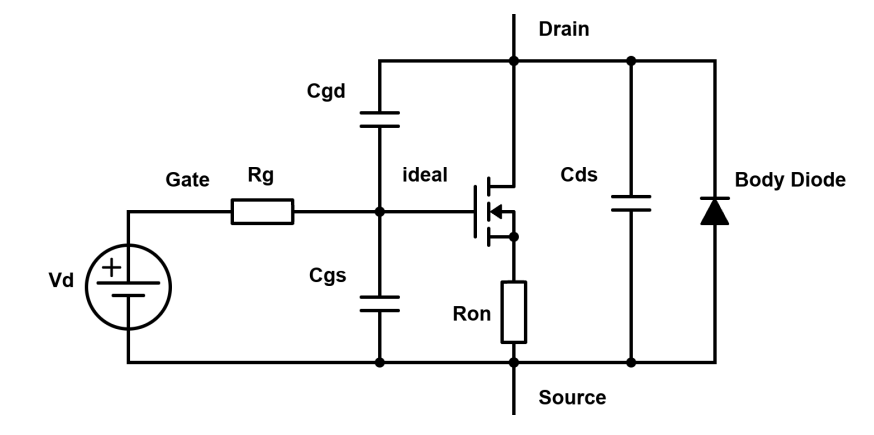
\includegraphics[width=0.75\linewidth]{Bilder//Kapitel2/GaNFET_ECM.png}
    \caption{Equivalent Circuit Model of a GaNFET}
    \label{fig:GaNFET_ECM}
\end{figure}
\subsubsection{Conductive Losses}
The conductive losses arise directly by the resistive impedance of the \ac{GaNFET} $R_{DS_{on}}$ during on-time. The current flowing through the \ac{HS} \ac{GaNFET} is equal to the current through the inductor during the charging phase $t_1$ and has the shape of a raised saw tooth wave. Calculating the \ac{RMS} value of the current necessary for the power calculation can be done with the equation \ref{eq:rms_raised_saw_tooth}. 
\begin{equation}
    I_{rms} = \sqrt{\frac{t_{on}}{T_s} \cdot \left( I_{min}\cdot I_{max}+\frac{\left(I_{max}-I_{min}\right)^2}{3}\right)} \label{eq:rms_raised_saw_tooth}
\end{equation}
The minimum and maximum currents through the \ac{GaNFET}, are equal to the minimum and maximum inductor currents $(I_{out}-\frac{\Delta I_{L_r}}{2})$ and $(I_{out}+\frac{\Delta I_{L_r}}{2})$. Their difference is directly expressed by the amplitude of the ripple current $\Delta I_{L_r}$. Inserting this and accounting for the duty cycle results in equation \ref{eq:rms_HS_GAN_1}. This simplifies to equation \ref{eq:rms_HS_GAN_2}. 
\begin{align}
    I_{rms_{HS}} &= \sqrt{\frac{T_s\cdot D}{T_s} \cdot \left(\left(I_{out}-\frac{\Delta I_{L_r}}{2}\right)\cdot \left(I_{out}+\frac{\Delta I_{L_r}}{2}\right)+\frac{\left(I_{L_r}\right)^2}{3}\right)}\label{eq:rms_HS_GAN_1}\\
    &=\sqrt{D \cdot \left(I_{out}^2 - \frac{\Delta I_{L_r}^2}{12}\right)}\label{eq:rms_HS_GAN_2}
\end{align}
Since the power loss over a resistor is equal to the resistors value times the square of the current, the resulting conduction power loss for the \ac{HS} \ac{GaNFET} is expressed by equation \ref{eq:Pon_HS_GAN}. As the \ac{LS} \ac{GaNFET} experiences the falling edge of the inductors current, the minimum and maximum currents are identical to the \ac{HS}. The \ac{LS} conduction losses thereby follow the same form, only differing in the on-time fraction being $\left(1-D\right)$.
\begin{align}
    P_{con,HS} &= R_{ds_{on}} \cdot D \cdot \left(I_{out}^2 - \frac{\Delta I_{L_r}^2}{12}\right)\label{eq:Pon_HS_GAN}\\
    P_{con,LS} &= R_{ds_{on}} \cdot \left(1-D\right) \cdot \left(I_{out}^2 - \frac{\Delta I_{L_r}^2}{12}\right)\label{eq:Pon_LS_GAN}
\end{align}
Conduction losses are therefore only indirectly dependent on frequency, as the amplitude of the ripple current is frequency-dependent. However, in normal operation $I_{out}^2 >> \frac{\Delta I_{L_r}^2}{12}$, allowing the \ac{RMS} current to be approximated by the product of duty cycle and output current, removing the frequency dependence. 
\subsubsection{Dead Time Losses}
During both dead times, a current is conducted by the \ac{LS} \ac{GaNFET} via its "body diode", as it has a higher potential at its source than at its drain. As long as $t_{df}, t_{dr} << T_s$ the current during the dead time can be approximated to be constant. For the falling edge dead time $t_{df}$ this results in the maximum inductor current $(I_{out}+\frac{\Delta I_{L_r}}{2})$ flowing through the "body diode". The energy lost during this dead time is the momentary power loss given as the product of this current and the voltage across the diode $V_D$ times the duration of the dead time $t_{df}$ and is given by equation \ref{eq:dead_time_energy}. 
\begin{equation}\label{eq:dead_time_energy}
    E_{t_{df}} = V_D \cdot (I_out + \Delta I_{L_r}^2) \cdot t_{df}
\end{equation}
As this energy is lost every switching cycle, the over all falling edge dead time power loss is the energy multiplied by the switching frequency $f_s$. The same approach is used for the rising edge dead time $t_{dr}$. Here the current is the minimum inductor current $(I_{out}-\frac{\Delta I_{L_r}}{2})$ and the duration changes to $t_{dr}$. Summing up both dead time losses and factoring out the voltage and switching frequency, as they stay constant for both cases, the total dead time power loss is given by equation \ref{eq:dead_time_power_loss}.
\begin{equation}\label{eq:dead_time_power_loss}
P_{td} = V_D \cdot f_s \cdot \left(t_{df} \cdot \left(I_{out} + \Delta I_{L_{pp}}^2\right) + t_{dr} \cdot \left(I_{out} - \Delta I_{L_{pp}}^2\right)\right)    
\end{equation}
The source-drain $V_{sd}$ for \acp{GaNFET} is usually higher than the body diode voltage drop in \acp{MOSFET}, increasing the importance of minimizing dead time in \ac{GaNFET} \ac{SMPS}. \\

\subsubsection{Switching Losses}

Switching losses are differentiated between \textit{hard switching}, where the power losses are high, and \textit{soft switching}, where the power losses are close to zero. \textit{Hard switching} is analysed first to explain how switching losses occur and how \textit{soft switching} can minimize the losses.\\
In \acp{GaNFET}, during the transition between non-conducting and conducting, both a high current flows through it and a high voltage drop occurs. This results in power loss in the switch. To simplify the calculations, we assume the voltages and currents rise and fall linearly. Figures \ref{fig:MOSFET_transient_turnon} and \ref{fig:MOSFET_transient_turnoff} show the separate stages of the switching process at turn-on and turn-off.
\begin{figure}[H]
    \centering
    \begin{minipage}{0.5\textwidth}
        \centering
        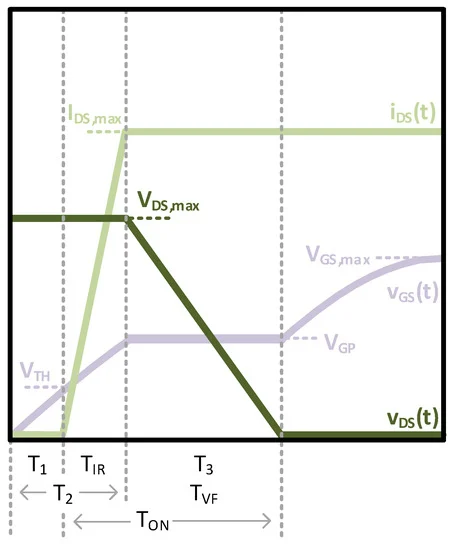
\includegraphics[width=0.7\linewidth]{Bilder/Kapitel2/MOSFET Transient turnon.png}
        \caption{Turn-On Transients}
        \label{fig:MOSFET_transient_turnon}
    \end{minipage}\hfill
    \begin{minipage}{0.5\textwidth}
        \centering
        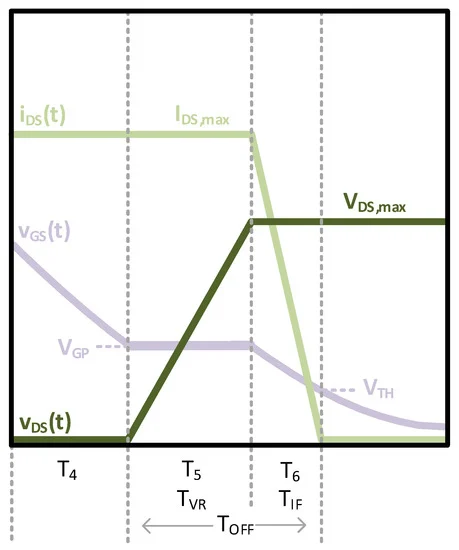
\includegraphics[width=0.7\linewidth]{Bilder/Kapitel2/MOSFET Transient turnoff.png}
        \caption{Turn-Off Transients}
        \label{fig:MOSFET_transient_turnoff}
    \end{minipage}\hfill
\end{figure}
Stepping through the turn-on transient phases, the gate voltage increases, charging the gate-source capacitance $C_{gs}$. As soon as the threshold voltage $V_{th}$ is reached, the \ac{GaNFET} begins to conduct. The gate voltage continues increasing, leading to a rise in the current $I_{ds}$ through the switching element. The drain-source voltage $V_{ds}$ stays constant as the gate-source capacitance $C_{gs}$ is not yet able to discharge through the \ac{GaNFET}. $I_{ds}$ and $V_{gs}$ continue to rise, until the gate-source voltage reaches the miller plateau. At this point, $C_{gd}$ and $C_{gs}$ are effectively connected in parallel, which increases the overall gate capacitance. Furthermore, $C_{gd}$ is charged with a large negative voltage, when compared to $C_{gs}$, resulting in the entire gate current $I_g$ being used to discharge the capacitor. Thereby, $C_{gs}$ cannot continue charging until $C_{gd}$ has reached the same potential. On the other hand, $V_g$ also cannot drop below $V_{pl}$, as this would cause $C_{dg}$ to no longer be able to discharge and $V_g$ to rise to $V_{pl}$ again. As a result, $V_g$ stays constant until $C_{gd}$ has reached the potential of $C_{gs}$. The voltage $V_{ds}$ decreases during this time, as both $C_{gd}$ and $C_{ds}$ are able to discharge. As $V_{ds}$ hits zero, the gate voltage starts to increase again.\\
On turn-off, the same procedure takes place only this time in reverse. The gate voltage $V_g$ decreases as $V_d$ is set to zero until the miller plateau is reached. Here the output capacitances $C_{gd}$ and $C_{ds}$ begin to charge up again, raising the drain-source voltage $V_{ds}$ until they are fully charged. After this, the current begins to drop together with $V_g$ until the threshold voltage $V_{th}$ is reached and the current is equal to zero.\\\\
The energy lost per cycle through turn-on and turn-off is equal to the area of the triangle formed by the product of $V_{ds}(t)$ and $I_{ds}(t)$. Multiplying this by the frequency of cycles $f_s$ gives the total power shown in equation \ref{eq:switching_power}.
The maximum voltages of the transient process are assumed to be constant, since the time of one switching Period $T_s >> t_{on},t_{off}$. For the HS switching element, both at turn-on and turn-off the voltage $V_{ds,max}$ is equal to $V_{in}$. The current, however, differs for the two cases as the inductor current, and thereby the current through the switching element is rising during the on period. At turn-on $I_{ds,max}$ is equal to $(I_{out} - \frac{\Delta I_{L_{pp}}}{2})$ and at turn-off equal to $(I_{out} + \frac{\Delta I_{L_{pp}}}{2})$. Because of this, the total power loss of the HS switching element through switching losses is:
\begin{align}
    P_{s,HS} &= f_s \cdot \frac{1}{2} \cdot V_{ds,max} \cdot I_{in,max} \cdot t_{on,off}\label{eq:switching_power} \\
    &= f_s \cdot \frac{1}{2} \cdot V_{in} \cdot \left[t_{on} \cdot \left(I_{out} - \frac{\Delta I_{L_{pp}}}{2}\right) + t_{off} \cdot \left(I_{out} + \frac{\Delta I_{L_{pp}}}{2}\right)\right]
\end{align}
For the LS switching element, this equation only partially holds, as here the switching does not occur as \textit{hard switching} but as \textit{soft switching}. Ideal \textit{soft switching} comes in the form of \textit{\ac{ZVS}}, \textit{\ac{ZCS}} or a combination of both (ZVZCS). For \ac{ZVS} at turn-on the voltage $V_{ds}$ is discharged before the current begins to rise, effectively creating no region where both $V_{ds}$ and $I_{ds}$ are greater than zero. Since there is no overlap, the power loss is zero, eliminating switching power loss. For turn-off, the same ideal holds for \ac{ZCS}, as letting $I_{ds}$ first drop to zero and then increasing $V_{ds}$ results in zero losses. While ideal soft switching can eliminate switching losses, this is not necessary for something to be considered soft switching. In non-ideal soft switching, the current or voltage is lower than in the hard switching case however, it does not equal zero.\\
This is the case for the \ac{LS} switching element. Since its "body diode", as depicted in figure \ref{fig:GaNFET_ECM}, is pointing in the direction of the current and conducting before turn-on, the voltage $V_{ds}$ is equal to the forward voltage of this "body diode" $V_D$.
\begin{equation}
    V_{ds} = V_D << V_{in}
\end{equation}
Instead of having to lower the voltage from $V_{in}$ to zero during turn-on, it only needs to be lowered from $V_D$, in turn shortening the miller plateau and lowering the product of $I_{ds}$ and $V_{ds}$.
On turn-off, this also holds true, as only $V_D$ needs to be reached. This lowers the switching losses of the \ac{LS} switching element significantly and can therefore be neglected in many cases. To calculate the \ac{LS} switching losses, the same equation \ref{eq:switching_power} as used for the \ac{HS} switching losses is used. Substituting the input voltage $V_{in}$ by the diode voltage $V_D$ and swapping the currents experienced at turn-on and turn-off, yields equation \ref{eq:switching_power_LS}.
\begin{equation}\label{eq:switching_power_LS}
    P_{s,LS} = f_s \cdot \frac{1}{2} \cdot V_D \cdot (t_{on} \cdot (I_{out} + \frac{\Delta I_{L_{pp}}}{2}) + t_{off} \cdot (I_{out} - \frac{\Delta I_{L_{pp}}}{2}))    
\end{equation}
In comparison with the switching losses of the \ac{HS} switching element, here the current at turn-on and turn-off are switched since turn-on for the low side is directly after turn-off of the high side and vice versa for turn-off on the low side.
\subsubsection{Switching element combined losses}
Superposing the discussed types of losses results in a clear frequency dependence. For low switching frequencies, the conductive losses outweigh the dead time and switching losses. At higher frequencies, a linear correspondence between losses and frequency is to be expected. 

\subsection{Losses in the inductor} \label{sec:losses_in_the_inductor}
Concerning inductors, two kinds of losses are differentiated. The losses created by the resistance of the spool are called winding losses, while core losses describe the losses appearing in the core of the inductor. First, the winding losses will be explained, followed by the hysteresis losses of the inductors core.

\subsubsection{Winding losses}
The spool's resistance consists of a base DC resistance which is altered by the frequency-dependent skin effect and proximity effect. The momentary power is then calculated by taking the square of the current through the inductor and multiplying it with this resistance. 
\begin{equation}
    P_{L_{W}}(t) = R(f) \cdot I_L(t)^2
\end{equation}
The average power is then determined by taking the integral of the momentary power and dividing it by the elapsed time.
\begin{equation}
    P_{L_{W}} = \frac{1}{T} \int_{0}^{T} R(f) \cdot I_L(t)^2 dt    
\end{equation}
Losses in the core have two main causes, Eddy currents and Hysteresis. The inductor in the buck converter is subjected to a changing magnetic field. That changing magnetic field induces a voltage in the core, following Faraday's law. According to Lenz's law, this voltage results in a current in the core of the inductor that is opposed to the creating current. These currents form circular paths, hence eddy currents. Considering highly conductive core materials like metal alloys, the low ohmic resistance effectively creates a short and a high current is able to flow resulting in considerate losses. Changing the core material to have a higher resistance, lowering the induced current or splitting the core into many different slices lowering the induced voltage per slice, decreases the core losses resulting from eddy currents. Power inductor cores consisting of powder ferrite or composite materials moulded into the desired shape, provide a high ohmic resistance, as the individual powder particles are insulated from one another.

\subsubsection{Hysteresis losses}
The second type of core loss, hysteresis loss, originates from the core's magnetisation. A non-magnetized core consists of many macroscopic regions of different magnetization. The magnetic moments in one of these regions called magnetic domains are all oriented in the same direction and are separated from the other domains by domain walls only a few hundred atoms wide. When an external magnetic field $H$ is applied to the core, the magnetic domains oriented in the direction of this field expand, shifting the domain walls and increasing the magnetic flux density $B$ in the core. At a certain point, the core becomes saturated, as the domains can only expand further in some regions of the inductor. This explains, why the relationship between the magnetic field strength $H$ and the B-field in an inductor is non-linear. When the current through the inductor and thereby its magnetic field strength decreases, the magnetic flux density also decreases. Depending on the type of core material, the magnetic domains are easy or hard to return to a non-magnetized state. Magnetically hard materials like permanent magnets keep their magnetic flux density even if no external field is present. They have to be subjected to a strong opposing magnetic field, to be demagnitized. On the other hand, magnetically softer materials like steel easily decrease their magnetic flux density, with only a small amount of energy needed to return to a fully demagnetised state. This difference between the charging and discharging behaviour of an inductor is called hysteresis.\\
Plotting the relative B-H curve of an inductor as in figure \ref{fig:b-hcurve} displays this hysteresis, giving insight into the ease of magnetization, point of saturation and the energy stored and released by the inductor. 
The maximum B-field $B_{max}$, the remnant B-field $B_r$ and the coercivity $H_c$ are points of interest along this curve used in later chapters to characterize the inductor.
\begin{figure}[H]
    \centering
    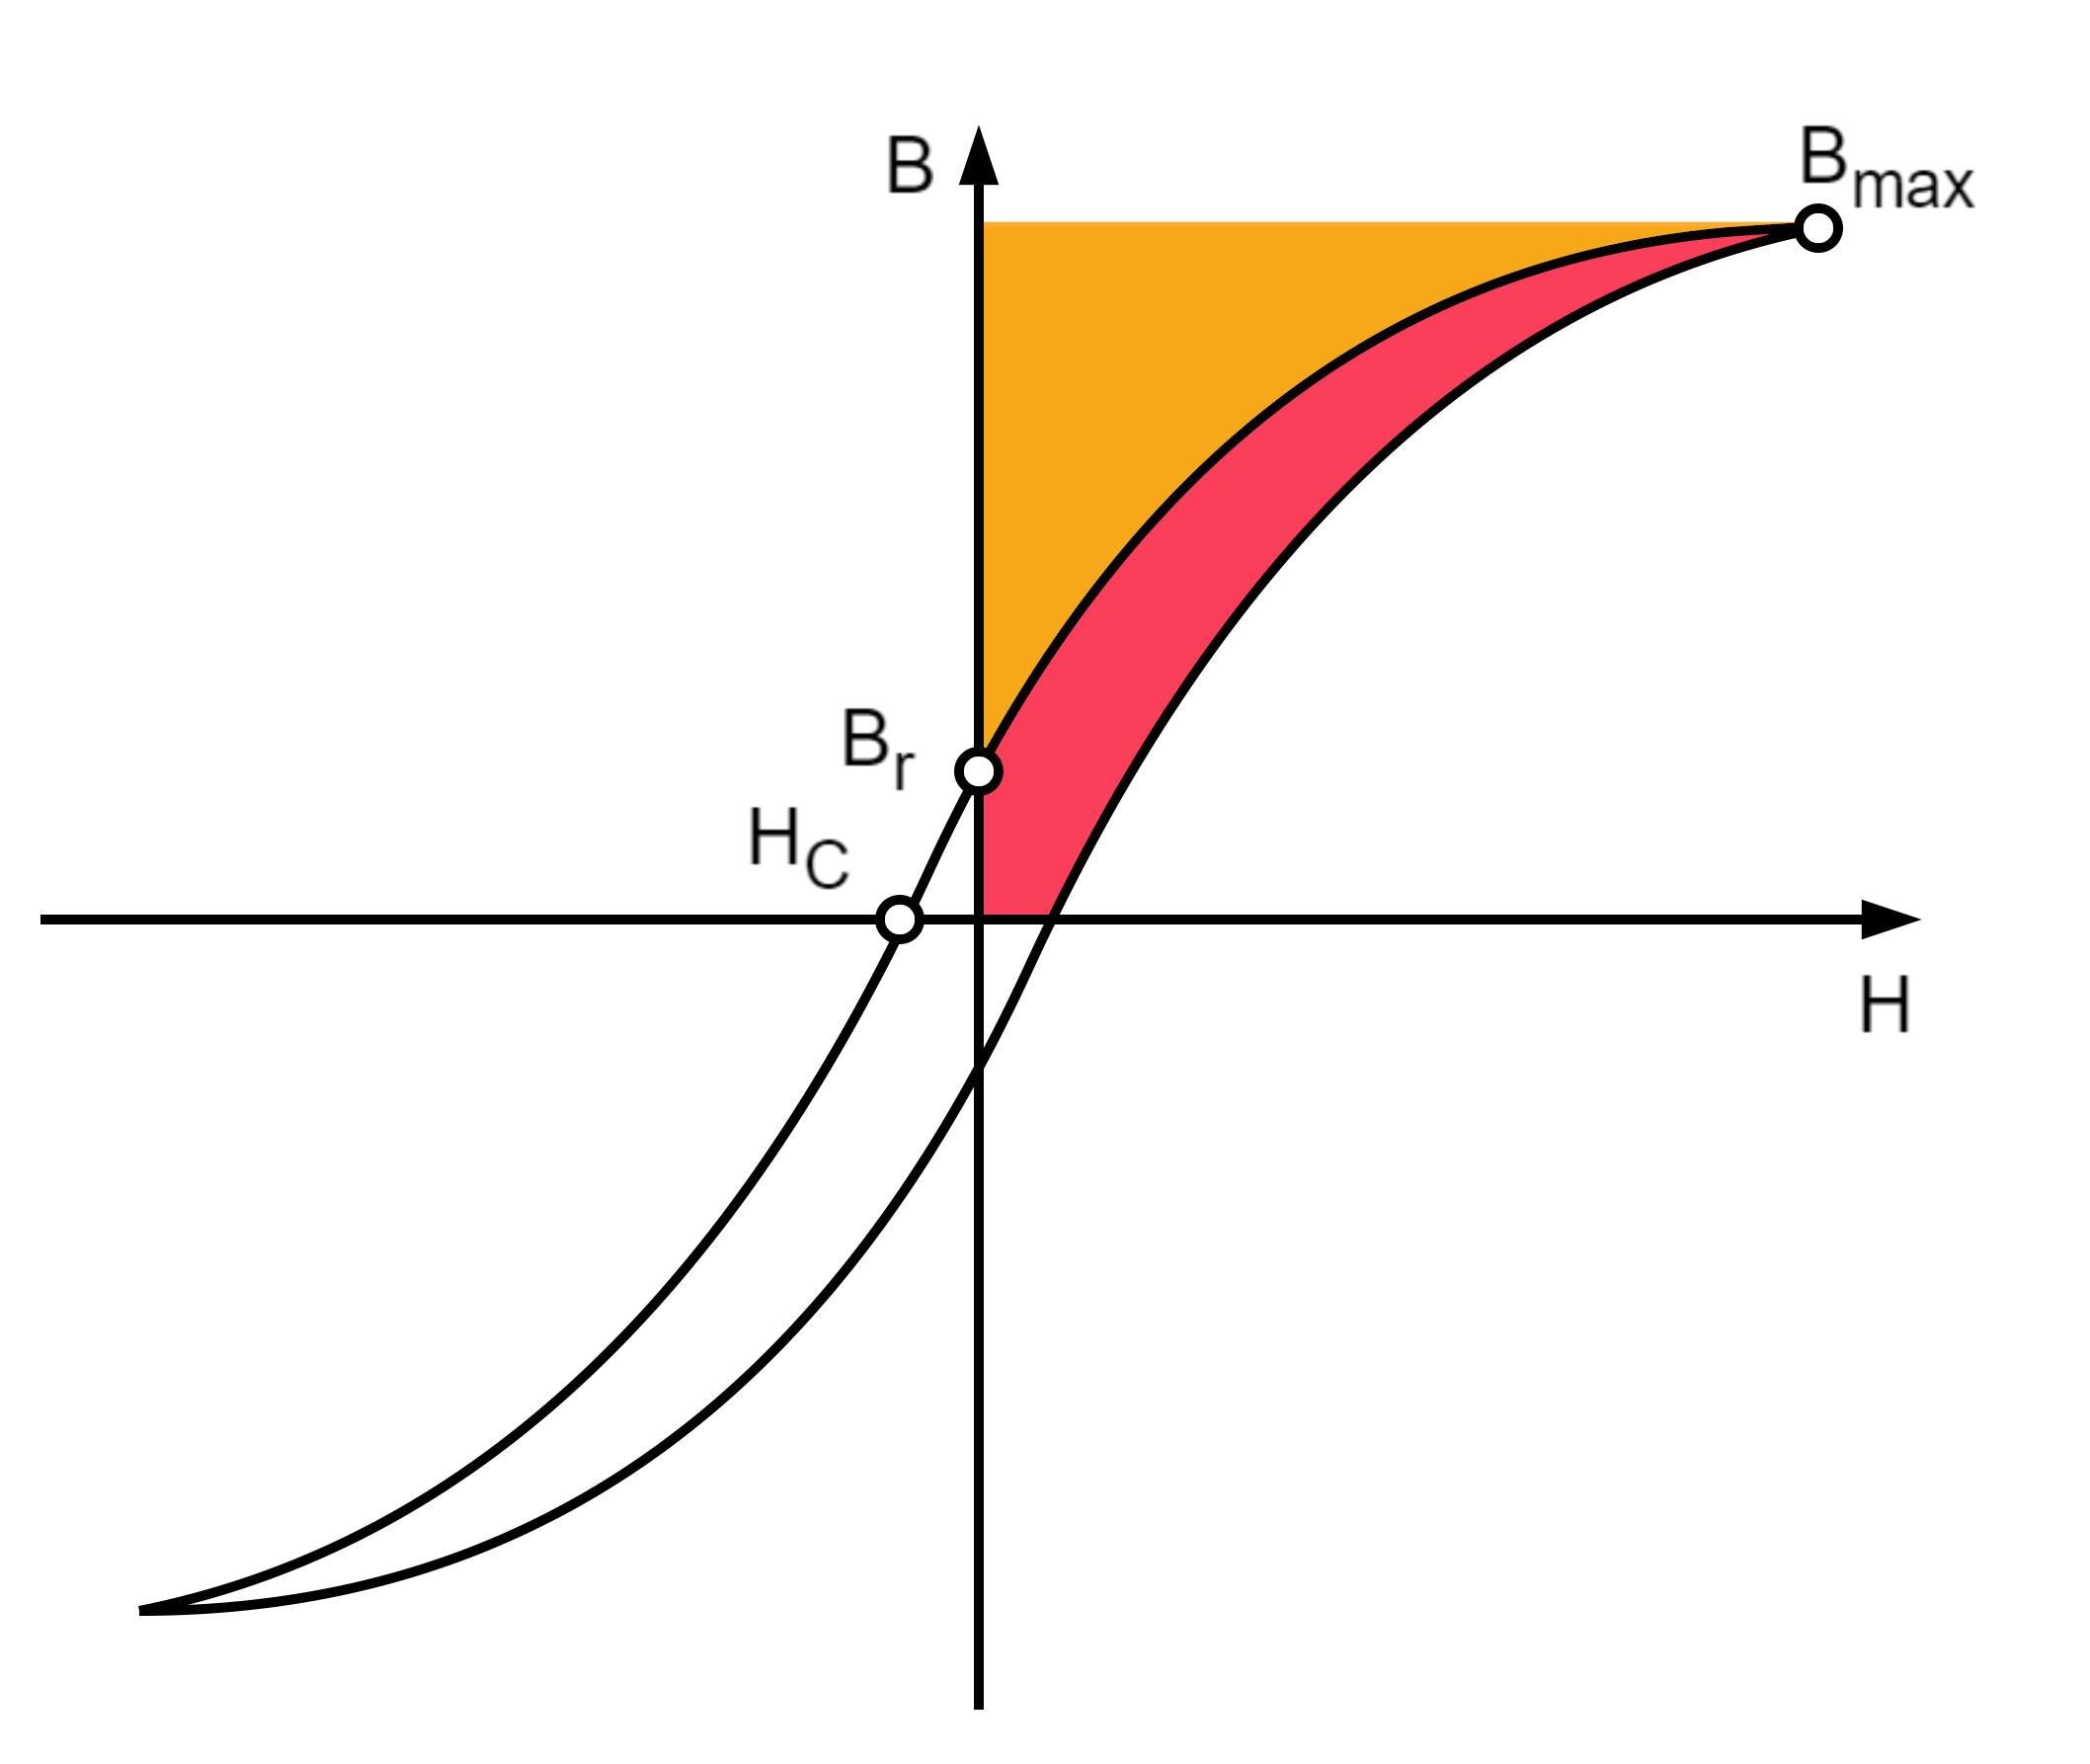
\includegraphics[width=0.6\linewidth]{Bilder//Kapitel2/Hysteresiscurve.png}
    \caption{Hysteresis Loop of a magnetically soft inductor core}
    \label{fig:b-hcurve}
\end{figure}
The energy put into the inductor to charge its B-field can be determined by calculating the area under the curve along the B-field as in equation \ref{eq:hysteresis_energy}. The same equation holds true for the energy released by the inductor when following the upper part of the curve.
\begin{equation}
        E = \int H dB \label{eq:hysteresis_energy}
\end{equation}
The energy lost through charging and discharging the inductor is their difference given as the cyclic integral along the two curves as shown in equation \ref{eq:hysteresis_energy_cyclic}.
\begin{equation}
    E_{loss} = \oint_{Loop} H dB \label{eq:hysteresis_energy_cyclic}
\end{equation}
In buck converters, we assume a constant DC current $I_L$ through the inductor superposed with a ripple current $I_{L_r}$. In accordance with Ampere's Law the momentary H-field is determined by the momentary current through the inductor. Operating with a continuous current through the inductor, the formation of hysteresis loops shown in figure \ref{fig:DC_Bias_Hysteresis} can be observed. 
\begin{figure}[H]
    \centering
    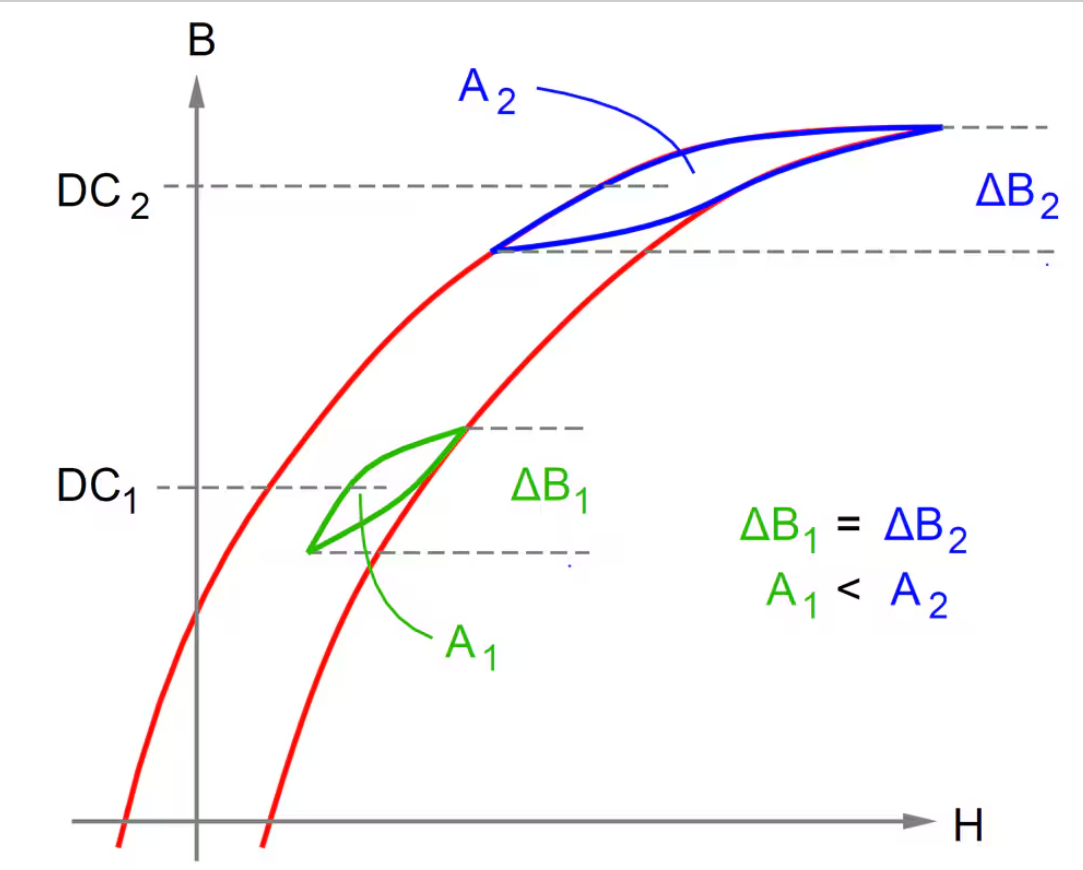
\includegraphics[width=0.4\linewidth]{Bilder//Kapitel2/DC_Bias_Hysteresis.png}
    \caption{Hysteresis Loop with different DC biases}
    \label{fig:DC_Bias_Hysteresis}
\end{figure}
The average H-field is determined by the DC current, while the amplitude of the ripple current determines the difference in the H-field $\Delta H$. The energy lost every cycle of the buck converter is equal to the area enclosed by this loop. The core loss due to hysteresis can therefore be determined by multiplying the area of the loop with the switching frequency.
\begin{equation}
    P_{Hys} = \oint_{Loop} H\left(B,f_s\right)  dB \cdot f_s
\end{equation}
It is important to take into consideration, that the loop size itself is dependent on the switching frequency as the ripple current amplitude is a function of the switching frequency. Therefore, the power lost due to hysteresis is not linearly proportional to the switching frequency, depending heavily on the amplitude of the ripple current.

With a high enough DC current, the inductor reaches saturation. Here, the Inductance $L$ decreases rapidly, increasing the ripple current amplitude and thereby also increasing the size of the hysteresis loop. Operating the buck converter while in saturation is not desirable, as it drastically increases the core losses.

%Herleitung für die Tatsache, dass bei Sättigung der Ripple Current größer wird
%\begin{align}
%    I &= \oint_C H ds = H\cdot\frac{l}{N}\\
%    \Phi &= B \cdot A_c\\
%    L &= \frac{\Phi}{I} = \frac{B}{H} \cdot \frac{N \cdot A_c}{l} \propto \frac{B}{H}\\
%    V_L &= L \cdot \frac{di}{dt} = L \cdot \frac{\Delta i}{\Delta t}\\
%    &\Rightarrow \Delta i \propto \frac{H}{B}
%\end{align}

%This process, called Barkhausen noise, is not continuous but happens in small jumps, as crystal defects, surface defects and further effects impede the domain wall movements. When the impedance is overcome the local magnetisation changes suddenly and a current is induced in the core material. 

%Quelle: 
% https://www.e-magnetica.pl/doku.php/magnetic_saturation#coercivity
% https://www.e-magnetica.pl/doku.php/magnetic_domain
% https://www.e-magnetica.pl/doku.php/domain_wall
% https://ieeexplore.ieee.org/stamp/stamp.jsp?tp=&arnumber=9617451
% https://www.e-magnetica.pl/doku.php/barkhausen_noise





%\section{Characterizing the Inductor}
%Since we are only going up to the first resonant frequency of the inductor, a simple equivalent circuit consisting of a parallel capacitor, two resistors, one in series and one in parallel and the inductor suffices in describing the frequency behaviour of the real inductor.
%\todo[inline]{What can be said about the inductor and how can this be inserted into LT Spice}
%\todo[inline]{Frequencybehaviour}
%\todo[inline]{Saturation}
%\todo[inline]{Hysteresis}




%\subsection{NOTES}
%Skindepth calculations with https://www.allaboutcircuits.com/tools/skin-depth-calculator/ :
%Copper at 4MHz: 32.60um  --> 0.0326mm
%Copper at 80kHz: 230.5um --> 0.235mm